\documentclass[12pt]{article}
\setlength\parindent{0pt}
\usepackage{amsmath}
\usepackage{lscape}
\usepackage{graphicx}
\usepackage{fullpage}
\usepackage[margin=0.8in]{geometry}
\setlength{\parskip}{4mm}
\def\LL{\left\langle}   % left angle bracket
\def\RR{\right\rangle}  % right angle bracket
\def\LP{\left(}         % left parenthesis
\def\RP{\right)}        % right parenthesis
\def\LB{\left\{}        % left curly bracket
\def\RB{\right\}}       % right curly bracket
\def\PAR#1#2{ {{\partial #1}\over{\partial #2}} }
\def\PARTWO#1#2{ {{\partial^2 #1}\over{\partial #2}^2} }
\def\PARTWOMIX#1#2#3{ {{\partial^2 #1}\over{\partial #2 \partial #3}} }
\newcommand{\BE}{\begin{displaymath}}
\newcommand{\EE}{\end{displaymath}}
\newcommand{\BNE}{\begin{equation}}
\newcommand{\ENE}{\end{equation}}
\newcommand{\BEA}{\begin{eqnarray}}
\newcommand{\EEA}{\nonumber\end{eqnarray}}
\newcommand{\EL}{\nonumber\\}
\newcommand{\la}[1]{\label{#1}}
\newcommand{\ie}{{\em i.e.\ }}
\newcommand{\eg}{{\em e.\,g.\ }}
\newcommand{\cf}{cf.\ }
\newcommand{\etc}{etc.\ }
\newcommand{\Tr}{{\rm tr}}
\newcommand{\etal}{{\it et al.}}
\newcommand{\OL}[1]{\overline{#1}\ } % overline
\newcommand{\OLL}[1]{\overline{\overline{#1}}\ } % double overline
\newcommand{\OON}{\frac{1}{N}} % "one over N"
\newcommand{\OOX}[1]{\frac{1}{#1}} % "one over X"
\pagenumbering{gobble}
\begin{document}
	\Large
\centerline{\sc{Quiz 3 -- The Seasons (retake)}}

\begin{minipage}{0.6\textwidth}
	\Large
	Name: \underline{\hspace{3in}}
\end{minipage}
\begin{minipage}{0.4\textwidth}
	\Large
	Lab Section: M0\underline{\hspace{1in}}\\
	\small (if you want your paper back)
\end{minipage}

\normalsize

	On the back of this page, you'll find a diagram of Earth similar to the one on your homework.  


\begin{enumerate}	
	\item Consider an observer on the Antarctic Circle.
	
	\begin{enumerate}
		\item Where would this observer see the Sun at noon on the December solstice? Draw a stick figure on the globe (oriented correctly with an arrow toward the Sun) to argue that your answer is correct.
		
		\vspace{1in}
		
		\item Where would this observer see the Sun at midnight on the December solstice? Draw a stick figure on the globe (oriented correctly with an arrow toward the Sun) to argue that your answer is correct.
		
		\vspace{1.5in}
		
	\end{enumerate} 
	
	\item An observer sees the Sun high in their northern sky at noon on the June solstice. Six months later, on the December solstice, they see the Sun high in their southern sky at noon.
	
	\vspace{1.5in}
	
	
	\begin{enumerate}
		\item Where on Earth is this person located? Mark this observer's possible location on Earth and label it ``2a''.
		
		\item Would this observer have more hours of daylight in December, more hours of daylight in June, or an equal amount in both? 
		
		\vspace{1.5in}
		
	\end{enumerate}
	
	
	
\end{enumerate}

\newpage
\begin{landscape}
	
	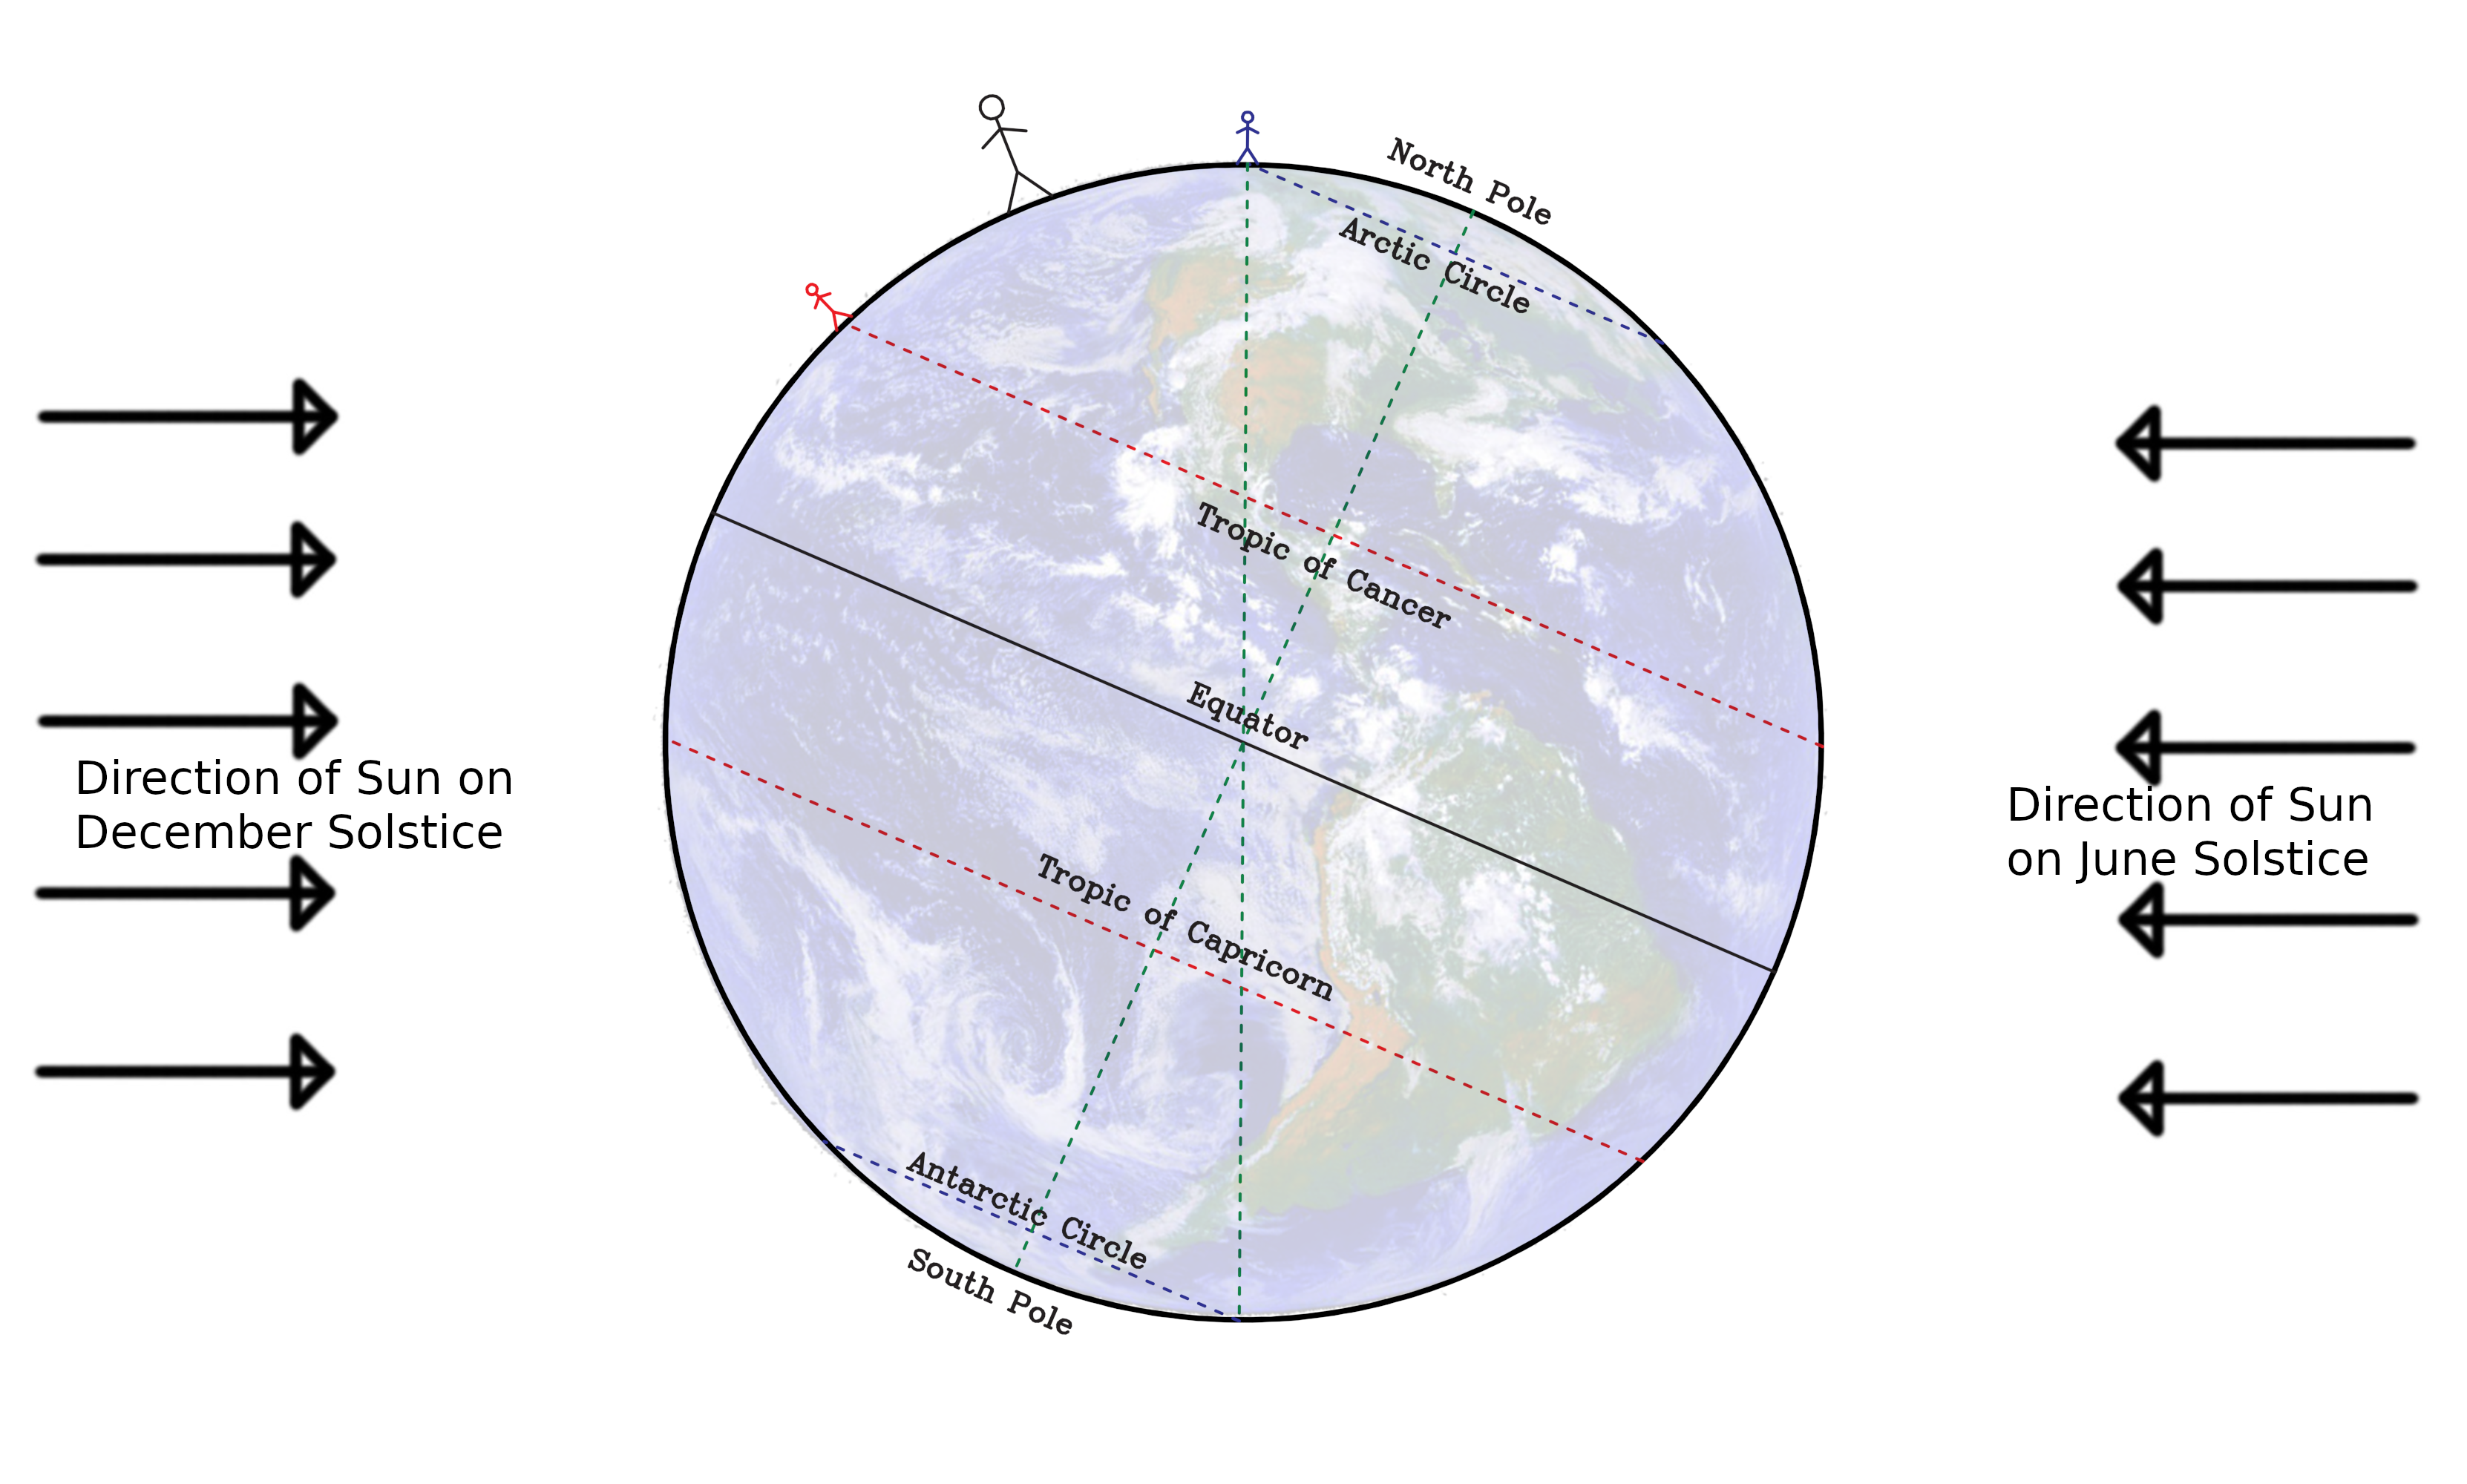
\includegraphics[width=10in]{earth-diagram-both.png}
	

	
\end{landscape}

	


\end{document}


